\documentclass{article}

% if you need to pass options to natbib, use, e.g.:
%     \PassOptionsToPackage{numbers, compress}{natbib}
% before loading neurips_2020

% ready for submission
\usepackage[preprint]{neurips_2020}

% to compile a preprint version, e.g., for submission to arXiv, add add the
% [preprint] option:
    % \usepackage[preprint]{neurips_2020}

% to compile a camera-ready version, add the [final] option, e.g.:
    % \usepackage[final]{neurips_2020}

% to avoid loading the natbib package, add option nonatbib:
    %  \usepackage[nonatbib]{neurips_2020}

\usepackage[utf8]{inputenc} % allow utf-8 input
\usepackage[T1]{fontenc}    % use 8-bit T1 fonts
\usepackage{hyperref}       % hyperlinks
\usepackage{url}            % simple URL typesetting
\usepackage{booktabs}       % professional-quality tables
\usepackage{amsfonts}       % blackboard math symbols
\usepackage{nicefrac}       % compact symbols for 1/2, etc.
\usepackage{microtype}      % microtypography
\usepackage{tikz}
\usepackage{amsmath,amssymb,amsthm}
\usepackage{fullpage,appendix,bm,graphicx}

\usepackage{pythonhighlight}
\usepackage[ruled,vlined,linesnumbered]{algorithm2e}


%%%%%%%%%%%%%%%%%%%%%%%%%%%%%%%%%%%%%%%%%%
% Custom commands                        %
%%%%%%%%%%%%%%%%%%%%%%%%%%%%%%%%%%%%%%%%%%

\newcommand{\vc}[1]{\boldsymbol{#1}}
\newcommand{\adj}[1]{\frac{d J}{d #1}}
\newcommand{\chain}[2]{\adj{#2} = \adj{#1}\frac{d #1}{d #2}}
\newcommand\norm[1]{\left\lVert#1\right\rVert}

% mathcal
\newcommand{\Ac}{\mathcal{A}}
\newcommand{\Bc}{\mathcal{B}}
\newcommand{\Cc}{\mathcal{C}}
\newcommand{\Dc}{\mathcal{D}}
\newcommand{\Ec}{\mathcal{E}}
\newcommand{\Fc}{\mathcal{F}}
\newcommand{\Gc}{\mathcal{G}}
\newcommand{\Hc}{\mathcal{H}}
\newcommand{\Ic}{\mathcal{I}}
\newcommand{\Jc}{\mathcal{J}}
\newcommand{\Kc}{\mathcal{K}}
\newcommand{\Lc}{\mathcal{L}}
\newcommand{\Mc}{\mathcal{M}}
\newcommand{\Nc}{\mathcal{N}}
\newcommand{\Oc}{\mathcal{O}}
\newcommand{\Pc}{\mathcal{P}}
\newcommand{\Qc}{\mathcal{Q}}
\newcommand{\Rc}{\mathcal{R}}
\newcommand{\Sc}{\mathcal{S}}
\newcommand{\Tc}{\mathcal{T}}
\newcommand{\Uc}{\mathcal{U}}
\newcommand{\Vc}{\mathcal{V}}
\newcommand{\Wc}{\mathcal{W}}
\newcommand{\Xc}{\mathcal{X}}
\newcommand{\Yc}{\mathcal{Y}}
\newcommand{\Zc}{\mathcal{Z}}

% mathbb
\newcommand{\Ab}{\mathbb{A}}
\newcommand{\Bb}{\mathbb{B}}
\newcommand{\Cb}{\mathbb{C}}
\newcommand{\Db}{\mathbb{D}}
\newcommand{\Eb}{\mathbb{E}}
\newcommand{\Fb}{\mathbb{F}}
\newcommand{\Gb}{\mathbb{G}}
\newcommand{\Hb}{\mathbb{H}}
\newcommand{\Ib}{\mathbb{I}}
\newcommand{\Jb}{\mathbb{J}}
\newcommand{\Kb}{\mathbb{K}}
\newcommand{\Lb}{\mathbb{L}}
\newcommand{\Mb}{\mathbb{M}}
\newcommand{\Nb}{\mathbb{N}}
\newcommand{\Ob}{\mathbb{O}}
\newcommand{\Pb}{\mathbb{P}}
\newcommand{\Qb}{\mathbb{Q}}
\newcommand{\Rb}{\mathbb{R}}
\newcommand{\Sb}{\mathbb{S}}
\newcommand{\Tb}{\mathbb{T}}
\newcommand{\Ub}{\mathbb{U}}
\newcommand{\Vb}{\mathbb{V}}
\newcommand{\Wb}{\mathbb{W}}
\newcommand{\Xb}{\mathbb{X}}
\newcommand{\Yb}{\mathbb{Y}}
\newcommand{\Zb}{\mathbb{Z}}

% mathbf lowercase
\newcommand{\av}{\mathbf{a}}
\newcommand{\bv}{\mathbf{b}}
\newcommand{\cv}{\mathbf{c}}
\newcommand{\dv}{\mathbf{d}}
\newcommand{\ev}{\mathbf{e}}
\newcommand{\fv}{\mathbf{f}}
\newcommand{\gv}{\mathbf{g}}
\newcommand{\hv}{\mathbf{h}}
\newcommand{\iv}{\mathbf{i}}
\newcommand{\jv}{\mathbf{j}}
\newcommand{\kv}{\mathbf{k}}
\newcommand{\lv}{\mathbf{l}}
\newcommand{\mv}{\mathbf{m}}
\newcommand{\nv}{\mathbf{n}}
\newcommand{\ov}{\mathbf{o}}
\newcommand{\pv}{\mathbf{p}}
\newcommand{\qv}{\mathbf{q}}
\newcommand{\rv}{\mathbf{r}}
\newcommand{\sv}{\mathbf{s}}
\newcommand{\tv}{\mathbf{t}}
\newcommand{\uv}{\mathbf{u}}
\newcommand{\vv}{\mathbf{v}}
\newcommand{\wv}{\mathbf{w}}
\newcommand{\xv}{\mathbf{x}}
\newcommand{\yv}{\mathbf{y}}
\newcommand{\zv}{\mathbf{z}}

% mathbf uppercase
\newcommand{\Av}{\mathbf{A}}
\newcommand{\Bv}{\mathbf{B}}
\newcommand{\Cv}{\mathbf{C}}
\newcommand{\Dv}{\mathbf{D}}
\newcommand{\Ev}{\mathbf{E}}
\newcommand{\Fv}{\mathbf{F}}
\newcommand{\Gv}{\mathbf{G}}
\newcommand{\Hv}{\mathbf{H}}
\newcommand{\Iv}{\mathbf{I}}
\newcommand{\Jv}{\mathbf{J}}
\newcommand{\Kv}{\mathbf{K}}
\newcommand{\Lv}{\mathbf{L}}
\newcommand{\Mv}{\mathbf{M}}
\newcommand{\Nv}{\mathbf{N}}
\newcommand{\Ov}{\mathbf{O}}
\newcommand{\Pv}{\mathbf{P}}
\newcommand{\Qv}{\mathbf{Q}}
\newcommand{\Rv}{\mathbf{R}}
\newcommand{\Sv}{\mathbf{S}}
\newcommand{\Tv}{\mathbf{T}}
\newcommand{\Uv}{\mathbf{U}}
\newcommand{\Vv}{\mathbf{V}}
\newcommand{\Wv}{\mathbf{W}}
\newcommand{\Xv}{\mathbf{X}}
\newcommand{\Yv}{\mathbf{Y}}
\newcommand{\Zv}{\mathbf{Z}}

% bold greek lowercase
\newcommand{\alphav     }{\boldsymbol \alpha     }
\newcommand{\betav      }{\boldsymbol \beta      }
\newcommand{\gammav     }{\boldsymbol \gamma     }
\newcommand{\deltav     }{\boldsymbol \delta     }
\newcommand{\epsilonv   }{\boldsymbol \epsilon   }
\newcommand{\varepsilonv}{\boldsymbol \varepsilon}
\newcommand{\zetav      }{\boldsymbol \zeta      }
\newcommand{\etav       }{\boldsymbol \eta       }
\newcommand{\thetav     }{\boldsymbol \theta     }
\newcommand{\varthetav  }{\boldsymbol \vartheta  }
\newcommand{\iotav      }{\boldsymbol \iota      }
\newcommand{\kappav     }{\boldsymbol \kappa     }
\newcommand{\varkappav  }{\boldsymbol \varkappa  }
\newcommand{\lambdav    }{\boldsymbol \lambda    }
\newcommand{\muv        }{\boldsymbol \mu        }
\newcommand{\nuv        }{\boldsymbol \nu        }
\newcommand{\xiv        }{\boldsymbol \xi        }
\newcommand{\omicronv   }{\boldsymbol \omicron   }
\newcommand{\piv        }{\boldsymbol \pi        }
\newcommand{\varpiv     }{\boldsymbol \varpi     }
\newcommand{\rhov       }{\boldsymbol \rho       }
\newcommand{\varrhov    }{\boldsymbol \varrho    }
\newcommand{\sigmav     }{\boldsymbol \sigma     }
\newcommand{\varsigmav  }{\boldsymbol \varsigma  }
\newcommand{\tauv       }{\boldsymbol \tau       }
\newcommand{\upsilonv   }{\boldsymbol \upsilon   }
\newcommand{\phiv       }{\boldsymbol \phi       }
\newcommand{\varphiv    }{\boldsymbol \varphi    }
\newcommand{\chiv       }{\boldsymbol \chi       }
\newcommand{\psiv       }{\boldsymbol \psi       }
\newcommand{\omegav     }{\boldsymbol \omega     }

% bold greek uppercase
\newcommand{\Gammav     }{\boldsymbol \Gamma     }
\newcommand{\Deltav     }{\boldsymbol \Delta     }
\newcommand{\Thetav     }{\boldsymbol \Theta     }
\newcommand{\Lambdav    }{\boldsymbol \Lambda    }
\newcommand{\Xiv        }{\boldsymbol \Xi        }
\newcommand{\Piv        }{\boldsymbol \Pi        }
\newcommand{\Sigmav     }{\boldsymbol \Sigma     }
\newcommand{\Upsilonv   }{\boldsymbol \Upsilon   }
\newcommand{\Phiv       }{\boldsymbol \Phi       }
\newcommand{\Psiv       }{\boldsymbol \Psi       }
\newcommand{\Omegav     }{\boldsymbol \Omega     }

\newtheorem{theorem}{Theorem}
\newtheorem{corollary}{Corollary}[theorem]
\newtheorem{lemma}[theorem]{Lemma}
\DeclareMathOperator*{\argmax}{arg\,max}
\DeclareMathOperator*{\argmin}{arg\,min}

\title{Label-Aware Attention for \\ Fine-Grained Emotion Detection}

\author{%
  Ethan Wu \\
  \texttt{yongyiw@andrew.cmu.edu} \\
   \And
   Yilin Wang \\
   \texttt{yilinwan@andrew.cmu.edu} \\
   \And
   Ziqi Liu \\
   \texttt{ziqil2@andrew.cmu.edu} \\
}

\begin{document}
\maketitle

\begin{abstract}
    Recognizing underlying emotions from plain text enables human to build more intelligent systems, abridging the gap between us and machines. Working on by far the largest manually annotated dataset for emotion detection GoEmotions, we propose a label-aware attention mechanism, where label semantics are leveraged to integrate contextualized representations and inform classification decisions. Combined with the class-balanced loss, our method improves the macro F1 score by 0.06 compared to the baseline classifier, achieving state-of-the-art performance on this emotion detection benchmark. \footnote{Data and code available at \href{https://github.com/yongyi-wu/nlp-group}{https://github.com/yongyi-wu/nlp-group}.}
\end{abstract}

\section{Introduction}\label{intro}
Emotion detection is one of the fundamental tasks for more advanced applications of Natural Language Processing and Human-Computer Interaction, ranging from dialog systems to spam detection. This task aims to assign emotion labels that could be easily understood by humans to given input texts. 

GoEmotions is a recent work that contains by far the largest manually annotated data of 58k English Reddit comments, labeled for 27 emotion categories or ``neutral'' \citet{demszky2020goemotions}. The baseline model proposed by the authors follows the conventional classification regime, where a pretrained language model (in this case, cased \textsc{Bert Base}) extracts the contextual representation of \texttt{[CLS]} token, which is then fed into a multilayer perceptron (MLP) to compute, for each emotion, the probability of existence in the given text. However, the fine-grained taxonomy in the GoEmotions dataset presents challenge for the baseline classifier to distinguish nuanced emotions, such as anger and annoyance, so the \texttt{[CLS]} token alone may not be able to carry enough information to yield desired performance across different labels. 

In this work, we propose a label-aware attention mechanism where each emotion (classification label) maintains its own latent representation, and uses it to query and aggregate the contextual representation of all tokens from the input text. By computing attention distribution for each emotion independently, we hope the semantic information carried by the label would guide the classifier to focus on different aspects of the same text. Our method is reminiscent of AttentionXML (\citet{you2019attentionxml}) and LEAM (\citet{wang2018joint}) but is much easier to implement and train by avoiding the probabilistic label tree or the temporal convolution. Our model is trained under the class-balanced loss proposed by  \citet{cui2019classbalanced}, which helped alleviate the uneven distribution of emotion labels in the GoEmotions dataset. 

% We have also tried another label-aware mechanism, which is inspired by the LEAM architecture (Wang et al. 2018). The detail of this model is presented in section \ref{rel}. The most significant distinction from our proposed model is this model's different computational approach towards making the classifier attending to different emotional aspects of the input text. By the time of submission, our proposed method wins out with the best performance in terms of overall macro-F1 score (the LEAM results are also presented in Section \ref{res}) and individual classes F1 scores. 

The paper is organized as follows: Section \ref{method} introduces the design of our proposed classifier. We then present experiment details Section \ref{exp} and show our method performs significantly better than the baseline. After that, we review related work in emotion detection in Section \ref{rel} and conclude our work with a discussion in Section \ref{conc}. 


\section{Related Work}\label{rel}

\paragraph{Emotion Detection Taxonomy}
Traditionally, researchers use two emotion categorization taxonomies: categorical and dimensional. On the categorical front, Ekman's model divides emotions into 6 fundamental categories (fear, disgust, surprise, joy, anger, sadness), while Plutchik's emotion wheels divide emotions into 8 fundamental types, with each being able to subdivide into subcategories. For dimensional approaches, emotion can be expressed continuously in two dimensions: valence (degree of positivity) and arousal (degree of intensity). GoEmotions dataset extends this traditional taxonomy to $27$ subcategories (excluding neutral), allowing models to learn more fine-grained distinctions between emotions in the corpora. 


% \subsection{Label Semantics}
\paragraph{LEAM} 
This model \citet{gaonkar2020modeling} deploys a different way to compute the attention weights of the emotion labels towards the input text. To help highlight the emotional information contained in different portions of the input text, instead of using the bilinear key-query attention mechanism as in our model, this approach uses the cosine similarity between each label representations (initialized by the BERT word embeddings of the label word) and each input word representations. The resultant signals are processed by a convolution layer followed by a max pool layer to extract the most salient similarity signal. Finally, we linearly transform the extracted signal and softmax to get the attention weights between label emotions and input words.

\paragraph{Extreme-scale Multi-label Classification}
In extreme-scale multi-label classification, it is a common practice to introduce label semantics to help model distinguish nuance between different classes (\citet{zhang2018deep}, \citet{you2019attentionxml}, \citet{chang2020taming}). AttentionXML builds a probabilistic label tree to perform classification in a divide-and-conquer fashion wherein a multi-label attention guides labels (or sets of labels) to focus on the most relevant part of a sentence. 

\paragraph{Modeling Label-semantic for predicting emotion reactions}
Gaonkar et al. found that adding the pretrained label semantics embeddings as input and incorporating the learned correlation between emotions in the loss function improves the performance over the baseline BERT model \citet{gaonkar2020modeling}. Augmenting this method and applying semi-supervised techniques on the unlabeled portion of ROCStories gives the SOTA model with F1-score being 65.88, which is 4.92 points higher than the baseline BERT model. 


\section{Method}\label{method} % Or "Methods", if you want to talk about algorithms?
\subsection{Overview}

Our proposed classifier consists of two modules, a label-aware attention and a multilayer perceptron, building on top of contextualized representations extracted by a pretrained language model. 

As illustrated in Figure \ref{fig:model}, each of emotion labels, denoted by superscripts $(0), (1), \cdots, (C)$, computes its attention weights to all tokens from the last layer of the language model. For each label, the aggregated vector representation is then concatenated with the representation of \texttt{[CLS]} to form a label-aware sentence embedding. Finally, this embedding is fed into a feedforward network to produce the score for each label. 

By allowing each label to attend to different components of a sentence, the label-aware attention enhances the expressiveness of the sentence embedding. Moreover, because the attention weights are computed independently for each label, similar to \citet{vaswani2017attention}, our method is embarrassingly parallelizable and easy to implement, capable of scaling to datasets with even more fine-grained annotation. 

We also attempt to alleviate the class unbalance problem in the GoEmotions dataset, by replacing the cross-entropy loss with the class-balanced (CB) loss proposed by \citet{cui2019classbalanced}. The CB loss addresses the class unbalance problem by up-weighting the mistakes in less common classes. 

\begin{figure}
\begin{center}
    \tikzset{every picture/.style={line width=0.75pt}} %set default line width to 0.75pt

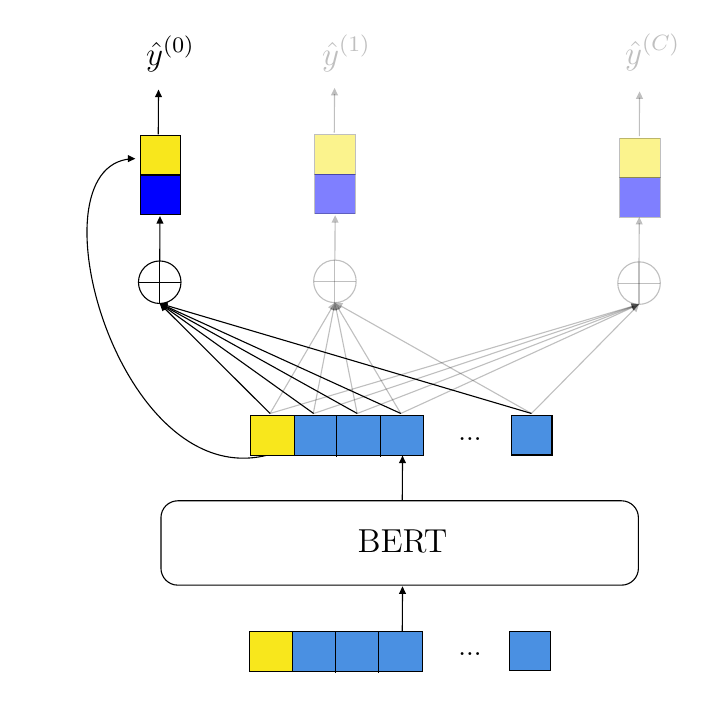
\begin{tikzpicture}[x=0.75pt,y=0.75pt,yscale=-1,xscale=1]
%uncomment if require: \path (0,440); %set diagram left start at 0, and has height of 440

%Straight Lines [id:da31370839057744115] 
\draw [color={rgb, 255:red, 0; green, 0; blue, 0 }  ,draw opacity=0.25 ]   (347.15,213.51) -- (396.86,163.08) ;
\draw [shift={(398.96,160.94)}, rotate = 134.59] [fill={rgb, 255:red, 0; green, 0; blue, 0 }  ,fill opacity=0.25 ][line width=0.08]  [draw opacity=0] (3.57,-1.72) -- (0,0) -- (3.57,1.72) -- cycle    ;
%Straight Lines [id:da20644252238970973] 
\draw [color={rgb, 255:red, 0; green, 0; blue, 0 }  ,draw opacity=0.25 ]   (284.17,213.51) -- (396.24,162.19) ;
\draw [shift={(398.96,160.94)}, rotate = 155.4] [fill={rgb, 255:red, 0; green, 0; blue, 0 }  ,fill opacity=0.25 ][line width=0.08]  [draw opacity=0] (3.57,-1.72) -- (0,0) -- (3.57,1.72) -- cycle    ;

%Straight Lines [id:da4987721771183171] 
\draw [color={rgb, 255:red, 0; green, 0; blue, 0 }  ,draw opacity=0.25 ]   (221.19,213.51) -- (250.92,162.69) ;
\draw [shift={(252.43,160.1)}, rotate = 120.32] [fill={rgb, 255:red, 0; green, 0; blue, 0 }  ,fill opacity=0.25 ][line width=0.08]  [draw opacity=0] (3.57,-1.72) -- (0,0) -- (3.57,1.72) -- cycle    ;
%Straight Lines [id:da39543032652670385] 
\draw [color={rgb, 255:red, 0; green, 0; blue, 0 }  ,draw opacity=0.25 ]   (347.15,213.51) -- (255.04,161.57) ;
\draw [shift={(252.43,160.1)}, rotate = 29.42] [fill={rgb, 255:red, 0; green, 0; blue, 0 }  ,fill opacity=0.25 ][line width=0.08]  [draw opacity=0] (3.57,-1.72) -- (0,0) -- (3.57,1.72) -- cycle    ;
%Straight Lines [id:da4699737293510331] 
\draw [color={rgb, 255:red, 0; green, 0; blue, 0 }  ,draw opacity=0.25 ]   (284.17,213.51) -- (253.96,162.68) ;
\draw [shift={(252.43,160.1)}, rotate = 59.28] [fill={rgb, 255:red, 0; green, 0; blue, 0 }  ,fill opacity=0.25 ][line width=0.08]  [draw opacity=0] (3.57,-1.72) -- (0,0) -- (3.57,1.72) -- cycle    ;
%Straight Lines [id:da5997958802161731] 
\draw [color={rgb, 255:red, 0; green, 0; blue, 0 }  ,draw opacity=0.25 ]   (263.18,213.51) -- (253.02,163.04) ;
\draw [shift={(252.43,160.1)}, rotate = 78.62] [fill={rgb, 255:red, 0; green, 0; blue, 0 }  ,fill opacity=0.25 ][line width=0.08]  [draw opacity=0] (3.57,-1.72) -- (0,0) -- (3.57,1.72) -- cycle    ;
%Straight Lines [id:da30720230167335916] 
\draw [color={rgb, 255:red, 0; green, 0; blue, 0 }  ,draw opacity=0.25 ]   (241.98,213.72) -- (251.86,163.04) ;
\draw [shift={(252.43,160.1)}, rotate = 101.03] [fill={rgb, 255:red, 0; green, 0; blue, 0 }  ,fill opacity=0.25 ][line width=0.08]  [draw opacity=0] (3.57,-1.72) -- (0,0) -- (3.57,1.72) -- cycle    ;

%Rounded Rect [id:dp9909194303175699] 
\draw   (168.63,263.71) .. controls (168.63,259.22) and (172.26,255.58) .. (176.75,255.58) -- (390.53,255.58) .. controls (395.02,255.58) and (398.66,259.22) .. (398.66,263.71) -- (398.66,288.09) .. controls (398.66,292.58) and (395.02,296.22) .. (390.53,296.22) -- (176.75,296.22) .. controls (172.26,296.22) and (168.63,292.58) .. (168.63,288.09) -- cycle ;
%Shape: Ellipse [id:dp8846878696918459] 
\draw   (157.79,150.27) .. controls (157.79,144.62) and (162.38,140.03) .. (168.04,140.03) .. controls (173.7,140.03) and (178.28,144.62) .. (178.28,150.27) .. controls (178.28,155.93) and (173.7,160.52) .. (168.04,160.52) .. controls (162.38,160.52) and (157.79,155.93) .. (157.79,150.27) -- cycle ;
%Straight Lines [id:da9716398351717932] 
\draw    (157.79,150.27) -- (178.28,150.27) ;
%Straight Lines [id:da6639959454699502] 
\draw    (168.04,140.03) -- (168.04,160.52) ;

%Shape: Ellipse [id:dp6966965234878091] 
\draw  [color={rgb, 255:red, 0; green, 0; blue, 0 }  ,draw opacity=0.25 ] (388.72,150.69) .. controls (388.72,145.04) and (393.31,140.45) .. (398.96,140.45) .. controls (404.62,140.45) and (409.21,145.04) .. (409.21,150.69) .. controls (409.21,156.35) and (404.62,160.94) .. (398.96,160.94) .. controls (393.31,160.94) and (388.72,156.35) .. (388.72,150.69) -- cycle ;
%Straight Lines [id:da26514083245396947] 
\draw [color={rgb, 255:red, 0; green, 0; blue, 0 }  ,draw opacity=0.25 ]   (388.72,150.69) -- (409.21,150.69) ;
%Straight Lines [id:da26578756686682437] 
\draw [color={rgb, 255:red, 0; green, 0; blue, 0 }  ,draw opacity=0.25 ]   (398.96,140.45) -- (398.96,160.94) ;

%Shape: Ellipse [id:dp6253805887233457] 
\draw  [color={rgb, 255:red, 0; green, 0; blue, 0 }  ,draw opacity=0.25 ] (242.19,149.86) .. controls (242.19,144.2) and (246.77,139.61) .. (252.43,139.61) .. controls (258.09,139.61) and (262.68,144.2) .. (262.68,149.86) .. controls (262.68,155.51) and (258.09,160.1) .. (252.43,160.1) .. controls (246.77,160.1) and (242.19,155.51) .. (242.19,149.86) -- cycle ;
%Straight Lines [id:da7602382209259668] 
\draw [color={rgb, 255:red, 0; green, 0; blue, 0 }  ,draw opacity=0.25 ]   (242.19,149.86) -- (262.68,149.86) ;
%Straight Lines [id:da0674775185762857] 
\draw [color={rgb, 255:red, 0; green, 0; blue, 0 }  ,draw opacity=0.25 ]   (252.43,139.61) -- (252.43,160.1) ;

%Curve Lines [id:da19895538466908347] 
\draw    (221.19,233.24) .. controls (148.43,253.65) and (104.68,95.04) .. (153.94,90.85) ;
\draw [shift={(156.25,90.77)}, rotate = 180.65] [fill={rgb, 255:red, 0; green, 0; blue, 0 }  ][line width=0.08]  [draw opacity=0] (3.57,-1.72) -- (0,0) -- (3.57,1.72) -- cycle    ;
%Straight Lines [id:da9633912521103427] 
\draw    (221.19,213.51) -- (170.16,162.64) ;
\draw [shift={(168.04,160.52)}, rotate = 44.91] [fill={rgb, 255:red, 0; green, 0; blue, 0 }  ][line width=0.08]  [draw opacity=0] (3.57,-1.72) -- (0,0) -- (3.57,1.72) -- cycle    ;
%Straight Lines [id:da9462664491194832] 
\draw    (242.19,213.51) -- (170.48,162.26) ;
\draw [shift={(168.04,160.52)}, rotate = 35.55] [fill={rgb, 255:red, 0; green, 0; blue, 0 }  ][line width=0.08]  [draw opacity=0] (3.57,-1.72) -- (0,0) -- (3.57,1.72) -- cycle    ;
%Straight Lines [id:da5464988488704245] 
\draw    (263.18,213.51) -- (170.66,161.98) ;
\draw [shift={(168.04,160.52)}, rotate = 29.11] [fill={rgb, 255:red, 0; green, 0; blue, 0 }  ][line width=0.08]  [draw opacity=0] (3.57,-1.72) -- (0,0) -- (3.57,1.72) -- cycle    ;
%Straight Lines [id:da7029151753238021] 
\draw    (284.17,213.51) -- (170.77,161.76) ;
\draw [shift={(168.04,160.52)}, rotate = 24.53] [fill={rgb, 255:red, 0; green, 0; blue, 0 }  ][line width=0.08]  [draw opacity=0] (3.57,-1.72) -- (0,0) -- (3.57,1.72) -- cycle    ;
%Straight Lines [id:da8906632189256127] 
\draw    (347.15,213.51) -- (170.91,161.37) ;
\draw [shift={(168.04,160.52)}, rotate = 16.48] [fill={rgb, 255:red, 0; green, 0; blue, 0 }  ][line width=0.08]  [draw opacity=0] (3.57,-1.72) -- (0,0) -- (3.57,1.72) -- cycle    ;
%Shape: Rectangle [id:dp3507359402768697] 
\draw  [fill={rgb, 255:red, 248; green, 231; blue, 28 }  ,fill opacity=1 ] (158.63,79.57) -- (178.2,79.57) -- (178.2,98.63) -- (158.63,98.63) -- cycle ;
%Shape: Rectangle [id:dp03364773196100135] 
\draw  [fill={rgb, 255:red, 0; green, 0; blue, 255 }  ,fill opacity=1 ] (158.63,98.63) -- (178.2,98.63) -- (178.2,117.69) -- (158.63,117.69) -- cycle ;
%Shape: Rectangle [id:dp46210527300453075] 
\draw  [fill={rgb, 255:red, 74; green, 144; blue, 226 }  ,fill opacity=1 ] (232.11,318.36) -- (294.46,318.36) -- (294.46,337.96) -- (232.11,337.96) -- cycle ;
%Straight Lines [id:da2128074768126642] 
\draw    (252.61,318.5) -- (252.61,338.56) ;
%Shape: Rectangle [id:dp6487133382547166] 
\draw  [fill={rgb, 255:red, 74; green, 144; blue, 226 }  ,fill opacity=1 ] (336.66,318.47) -- (356.22,318.47) -- (356.22,337.54) -- (336.66,337.54) -- cycle ;
%Straight Lines [id:da7615394976975725] 
\draw    (273.61,318.5) -- (273.61,338.56) ;
%Shape: Rectangle [id:dp05494384978133815] 
\draw  [fill={rgb, 255:red, 248; green, 231; blue, 28 }  ,fill opacity=1 ] (211.12,318.36) -- (232.11,318.36) -- (232.11,337.93) -- (211.12,337.93) -- cycle ;

%Straight Lines [id:da42222888162050465] 
\draw [color={rgb, 255:red, 0; green, 0; blue, 0 }  ,draw opacity=0.25 ]   (242.19,213.51) -- (396.12,161.89) ;
\draw [shift={(398.96,160.94)}, rotate = 161.46] [fill={rgb, 255:red, 0; green, 0; blue, 0 }  ,fill opacity=0.25 ][line width=0.08]  [draw opacity=0] (3.57,-1.72) -- (0,0) -- (3.57,1.72) -- cycle    ;
%Straight Lines [id:da6024765910505723] 
\draw [color={rgb, 255:red, 0; green, 0; blue, 0 }  ,draw opacity=0.25 ]   (221.19,213.51) -- (396.09,161.79) ;
\draw [shift={(398.96,160.94)}, rotate = 163.53] [fill={rgb, 255:red, 0; green, 0; blue, 0 }  ,fill opacity=0.25 ][line width=0.08]  [draw opacity=0] (3.57,-1.72) -- (0,0) -- (3.57,1.72) -- cycle    ;
%Straight Lines [id:da7725736479801701] 
\draw [color={rgb, 255:red, 0; green, 0; blue, 0 }  ,draw opacity=0.25 ]   (263.18,213.51) -- (396.17,162.02) ;
\draw [shift={(398.96,160.94)}, rotate = 158.84] [fill={rgb, 255:red, 0; green, 0; blue, 0 }  ,fill opacity=0.25 ][line width=0.08]  [draw opacity=0] (3.57,-1.72) -- (0,0) -- (3.57,1.72) -- cycle    ;
%Straight Lines [id:da8868304751030796] 
\draw    (284.89,255.43) -- (285,236.84) ;
\draw [shift={(285.01,233.84)}, rotate = 90.32] [fill={rgb, 255:red, 0; green, 0; blue, 0 }  ][line width=0.08]  [draw opacity=0] (3.57,-1.72) -- (0,0) -- (3.57,1.72) -- cycle    ;
%Straight Lines [id:da6008487533551252] 
\draw    (284.89,318.41) -- (285,299.82) ;
\draw [shift={(285.01,296.82)}, rotate = 90.32] [fill={rgb, 255:red, 0; green, 0; blue, 0 }  ][line width=0.08]  [draw opacity=0] (3.57,-1.72) -- (0,0) -- (3.57,1.72) -- cycle    ;
%Straight Lines [id:da899337147902147] 
\draw    (168.04,140.03) -- (168.14,121.44) ;
\draw [shift={(168.16,118.44)}, rotate = 90.32] [fill={rgb, 255:red, 0; green, 0; blue, 0 }  ][line width=0.08]  [draw opacity=0] (3.57,-1.72) -- (0,0) -- (3.57,1.72) -- cycle    ;
%Straight Lines [id:da8507680199625551] 
\draw [color={rgb, 255:red, 0; green, 0; blue, 0 }  ,draw opacity=0.25 ]   (252.43,139.61) -- (252.53,121.02) ;
\draw [shift={(252.55,118.02)}, rotate = 90.32] [fill={rgb, 255:red, 0; green, 0; blue, 0 }  ,fill opacity=0.25 ][line width=0.08]  [draw opacity=0] (3.57,-1.72) -- (0,0) -- (3.57,1.72) -- cycle    ;
%Straight Lines [id:da1747682258222547] 
\draw [color={rgb, 255:red, 0; green, 0; blue, 0 }  ,draw opacity=0.25 ]   (398.96,140.45) -- (399.07,121.86) ;
\draw [shift={(399.08,118.86)}, rotate = 90.32] [fill={rgb, 255:red, 0; green, 0; blue, 0 }  ,fill opacity=0.25 ][line width=0.08]  [draw opacity=0] (3.57,-1.72) -- (0,0) -- (3.57,1.72) -- cycle    ;
%Straight Lines [id:da05436810298257799] 
\draw    (167.33,79.09) -- (167.43,60.5) ;
\draw [shift={(167.45,57.5)}, rotate = 90.32] [fill={rgb, 255:red, 0; green, 0; blue, 0 }  ][line width=0.08]  [draw opacity=0] (3.57,-1.72) -- (0,0) -- (3.57,1.72) -- cycle    ;
%Shape: Rectangle [id:dp9332326457526785] 
\draw  [color={rgb, 255:red, 0; green, 0; blue, 0 }  ,draw opacity=0.25 ][fill={rgb, 255:red, 248; green, 231; blue, 28 }  ,fill opacity=0.5 ] (242.61,79.15) -- (262.17,79.15) -- (262.17,98.21) -- (242.61,98.21) -- cycle ;
%Shape: Rectangle [id:dp43512567814545333] 
\draw  [color={rgb, 255:red, 0; green, 0; blue, 0 }  ,draw opacity=0.25 ][fill={rgb, 255:red, 0; green, 0; blue, 255 }  ,fill opacity=0.5 ] (242.61,98.21) -- (262.17,98.21) -- (262.17,117.27) -- (242.61,117.27) -- cycle ;
%Shape: Rectangle [id:dp31911680926128727] 
\draw  [color={rgb, 255:red, 0; green, 0; blue, 0 }  ,draw opacity=0.25 ][fill={rgb, 255:red, 248; green, 231; blue, 28 }  ,fill opacity=0.5 ] (389.56,80.83) -- (409.13,80.83) -- (409.13,99.89) -- (389.56,99.89) -- cycle ;
%Shape: Rectangle [id:dp8655767183794414] 
\draw  [color={rgb, 255:red, 0; green, 0; blue, 0 }  ,draw opacity=0.25 ][fill={rgb, 255:red, 0; green, 0; blue, 255 }  ,fill opacity=0.5 ] (389.56,99.89) -- (409.13,99.89) -- (409.13,118.95) -- (389.56,118.95) -- cycle ;
%Straight Lines [id:da16085998336579554] 
\draw [color={rgb, 255:red, 0; green, 0; blue, 0 }  ,draw opacity=0.25 ]   (252.14,78.25) -- (252.25,59.66) ;
\draw [shift={(252.26,56.66)}, rotate = 90.32] [fill={rgb, 255:red, 0; green, 0; blue, 0 }  ,fill opacity=0.25 ][line width=0.08]  [draw opacity=0] (3.57,-1.72) -- (0,0) -- (3.57,1.72) -- cycle    ;
%Straight Lines [id:da007094542952027716] 
\draw [color={rgb, 255:red, 0; green, 0; blue, 0 }  ,draw opacity=0.25 ]   (399.1,79.93) -- (399.2,61.34) ;
\draw [shift={(399.22,58.34)}, rotate = 90.32] [fill={rgb, 255:red, 0; green, 0; blue, 0 }  ,fill opacity=0.25 ][line width=0.08]  [draw opacity=0] (3.57,-1.72) -- (0,0) -- (3.57,1.72) -- cycle    ;
%Shape: Rectangle [id:dp20108523415186186] 
\draw  [fill={rgb, 255:red, 74; green, 144; blue, 226 }  ,fill opacity=1 ] (232.91,214.36) -- (295.26,214.36) -- (295.26,233.96) -- (232.91,233.96) -- cycle ;
%Straight Lines [id:da9290869404007094] 
\draw    (253.41,214.5) -- (253.41,234.56) ;
%Shape: Rectangle [id:dp43464943110250087] 
\draw  [fill={rgb, 255:red, 74; green, 144; blue, 226 }  ,fill opacity=1 ] (337.46,214.47) -- (357.02,214.47) -- (357.02,233.54) -- (337.46,233.54) -- cycle ;
%Straight Lines [id:da5647307718463164] 
\draw    (274.41,214.5) -- (274.41,234.56) ;
%Shape: Rectangle [id:dp658752958965878] 
\draw  [fill={rgb, 255:red, 248; green, 231; blue, 28 }  ,fill opacity=1 ] (211.92,214.36) -- (232.91,214.36) -- (232.91,233.93) -- (211.92,233.93) -- cycle ;


% Text Node
\draw (158.52,28.5) node [anchor=north west][inner sep=2pt]  [font=\large] [align=left] {$\displaystyle \hat{y}^{( 0)}$};
% Text Node
\draw (285,275) node [anchor=center][inner sep=2pt]  [font=\large] [align=left] {{BERT}};
% Text Node
\draw (243.32,28.3) node [anchor=north west][inner sep=2pt]  [font=\large,color={rgb, 255:red, 0; green, 0; blue, 0 }  ,opacity=0.25 ] [align=left] {$\displaystyle \hat{y}^{( 1)}$};
% Text Node
\draw (389.32,27.9) node [anchor=north west][inner sep=2pt]  [font=\large,color={rgb, 255:red, 0; green, 0; blue, 0 }  ,opacity=0.25 ] [align=left] {$\displaystyle \hat{y}^{( C)}$};
% Text Node
\draw (309,222) node [anchor=north west][inner sep=2pt]   [align=left] {...};
% Text Node
\draw (309,326) node [anchor=north west][inner sep=2pt]   [align=left] {...};

\end{tikzpicture}
\end{center}

\caption{Visualization of the label-aware attention mechanism. The yellow block corresponds to the \texttt{[CLS]} token or its vector representation $\hv_1$.}
\label{fig:model}
\end{figure}

\subsection{Label-Aware Attention}

Given a tokenized text sequence $\xv$ of length $L$, we first obtain its contextualized representation from a pretrained language model: $\Hv = [\hv_1 \hv_2 \cdots \hv_L]^T \in \Rb^{L \times d}$, where $\hv_i$ is a $d$-dimensional vector representation for $i$-th token. 

For an emotion $i$, we maintain a trainable representation $\ev^{(i)} \in \Rb^{d'}$ and use it to query $\Hv$, where the attention scores are computed by bilinear products via a trainable matrix $\Wv \in \Rb^{d' \times d}$ to help align vector space of $\{\ev^{(i)}\}_{i = 1}^C$ and $\{\hv_j\}_{j = 1}^L$. Meanwhile, We omit linear projections of queries, keys and values as in \citet{vaswani2017attention}. A \texttt{softmax} layer is applied to the bilinear products to compute the attention weight distribution, 
$$\alpha_j^{(i)} = \texttt{softmax}\Bigl( \ev^{(i)T}\Wv_{\text{attn}}\hv_j \Bigr) = \frac{\exp(\ev^{(i)T} \Wv_{\text{attn}}  \hv_j)}{\sum_{k = 1}^L \exp(\ev^{(i)T} \Wv_{\text{attn}}  \hv_k)}$$
where $\alpha_j^{(i)}$ denotes the attention weight assigned by emotion $i$ to the $j$-th token. 

Finally, we aggregate the contextualized representations using weights computed above to obtain label-aware sentence representations (as indicated by dark blue boxes in Figure \ref{fig:model}): 
$$\tilde{\hv}^{(i)} = \sum_{k = 1}^L \alpha_k^{(i)} \hv_k.$$

\subsection{Classification Head}

While leveraging label semantics to pool last-layer representations from the pretrained language model, we do not waste the language model's intrinsic ability to extract sentence-level representation. Therefore, for an emotion $i$, we concatenate the label-aware sentence embedding $\tilde{\hv}^{(i)}$ with the typical embedding from \texttt{[CLS]} token $\hv_1$. The concatenated vector is passed into a MLP, which outputs the scalar probability that emotion $i$ exists in the input text: 
$$\hat{y}^{(i)} = \sigma\Bigl( \text{FFN}_i ([\tilde{\hv}^{(i)} \| \hv_1]) \Bigr).$$

We tie weights of classification head $\text{FFN}_{i}$ for all emotion $i$ to encourage the attention module to focus on different sets of contextualized embeddings in $\Hv$. This also prevents the classifier size grows linearly with respect to the number of labels. However, it is possible to inject stronger inductive bias and design specialized head for each label. We leave this idea for future works. 

\subsection{Class-Balanced Loss based on ENS}
In previous error analysis, we found that the baseline model often fails to distinguish low-resourced emotions from high-resourced emotions. This is an issue as the distribution of emotions in the goemotions dataset is unbalanced. To address this issue, we used the class-balanced loss introduced by \citet{cui2019classbalanced}. The effective number of samples (ENS) is defined as 
$
E_c = (1-\beta^{n_c}) / (1-\beta) 
$, where $\beta$ is a hyper-parameter (usually between 0.9 and 1) and $n_c$ is number of samples with emotion $c$. The class-balanced (CB) loss $\mathcal{L}_{CB}(p, y)$ weights the original loss by the ENS as follows:
$$
\mathcal{L}_{CB}(p, y) = \dfrac{1}{E_c} \mathcal{L} (p, y) = \dfrac{1-\beta}{1-\beta^{n_c}}\mathcal{L} (p, y)
$$
where $\mathcal{L} (p, y)$ is the cross entropy loss. 

\section{Experiments}\label{exp}
\subsection{Dataset}

\begin{figure}[h]
    \centering
    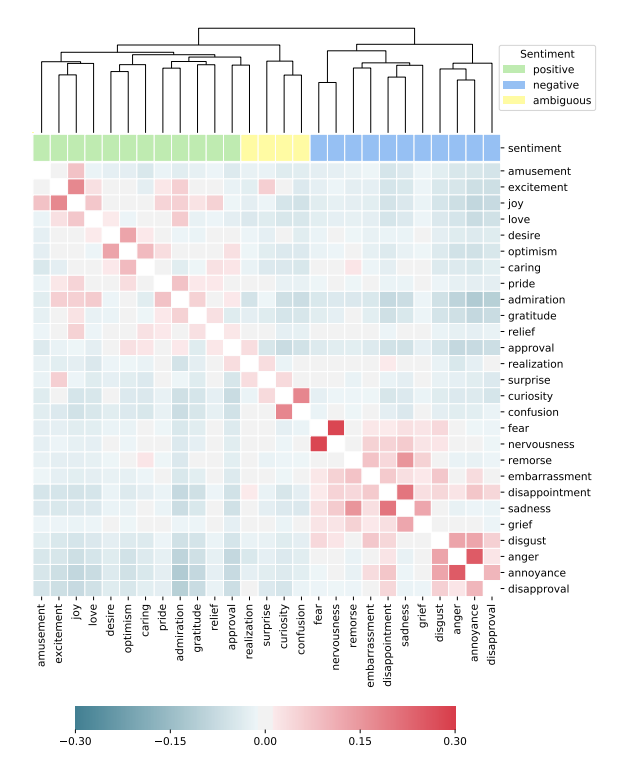
\includegraphics[width=8.4cm]{img/corr.png}
    \caption{Annotation results of the GoEmotions dataset. The heatmap shows the correlation between ratings for each emotion. The dendrogram represents the a hierarchical clustering of the ratings \citet{demszky2020goemotions}.}
\label{fig:corr}
\end{figure}


GoEmotions is a large dataset that consists of 58K English Reddit comments, each of which is labeled with one or more of 28 emotions (including ``neutral''). While GoEmotions characterizes a multi-label emotion classification task, most (83\%) of the samples have a single label. 


Despite some degree of inter-rater agreement, the heatmap from  Figure \ref{fig:corr} shows, some nuanced emotions, such as ``disgust'', ``anger'' ,and ``annoyance'' (bottom right corner), present even some annotation challenges. Such a fine-grained emotion taxonomy requires more a careful design of classifiers. 


\subsection{Model and Parameter}

To draw a fair comparison and demonstrate the benefit of label-aware attention, we use the same language model as \citet{demszky2020goemotions}, which is a pretrained cased \textsc{Bert Base}. The vector representation for each label is initialized to be a 768-dimensional word embedding of the corresponding emotion. However, the label representations are finetuned separately from the word embedding. Finally, the feedforward network in the classification head is a single linear layer with a bias term. 

When finetuning the pretrained \textsc{Bert} model, we use the same set of hyperparameters as \citet{demszky2020goemotions}. Specifically, the batch size is 16 and the learning rate is 5e-5 with the slanted triangular scheduler. For the CB loss, we choose $\beta = 0.95$. The finetuning is run for 4 epochs with no parameter held frozen. We run 10 experiments for each model under different seeds, and we average the performance over 10 experiments. 

\subsection{Results}\label{sec:res}
% \subsection{Model Statistics}
In Table \ref{tab:res}, we see that our model, which is equipped with label-aware attention (LAA) mechanism and trained under class-balanced (CB) loss, outperforms the baseline model. The Marco-average F1 of our model is 0.06 higher than that of the baseline model. Moreover, our model shows much lower variance under different seeds, which is an indication of robust design.


Aside from our best model, we also run two experiments which respectively involve LAA and LEAM only, and the results are presented in Appendix Table \ref{tab:full}. We see that our three models all outperform the baseline model, and the use of CB loss improved performance for the LAA model. 

\begin{table}[h]
    \begin{center}
    \begin{tabular}{|l |c| c|}
        \hline
         $\quad \quad \quad$ \textbf{Emotions} $\quad \quad \quad$ &  $\quad \quad \quad $ \textbf{Baseline}  $\quad \quad \quad $ & \textbf{LAA w/ CB Loss (ours)} \\ % &LEAM w/CE Loss\\
        \hline\hline
        Admiration &  0.65 & \textbf{0.67} \\
        Amusement & 0.80 & \textbf{0.81} \\
        Anger & 0.47 &\textbf{0.49} \\
        Annoyance & 0.34 &\textbf{0.37}\\
        Approval & 0.36 & \textbf{0.41}\\
        Caring & 0.39 & \textbf{0.43} \\
        Confusion & 0.37 &\textbf{0.42} \\
        Curiosity & 0.54 & \textbf{0.56}\\
        Desire & \textbf{0.49} & \textbf{0.49}\\
        Disappointment & 0.28 &\textbf{0.33} \\
        Disapproval & 0.39 & \textbf{0.41} \\
        Disgust & 0.45 & \textbf{0.48} \\
        Embarrassment & 0.43 &\textbf{0.45}\\
        Excitement & 0.34 & \textbf{0.41}\\
        Fear &  0.60 & \textbf{0.67} \\
        Gratitude & 0.86 & \textbf{0.90}\\
        Grief & 0.00 & \textbf{0.42}\\
        Joy & 0.51 & \textbf{0.60}\\
        Love & 0.78 & \textbf{0.79} \\
        Nervousness & \textbf{0.34} & \textbf{0.34} \\
        Neutral & \textbf{0.68} & 0.67\\
        Optimism & 0.51 & \textbf{0.56}\\
        Pride &  0.36 & 0.49\\
        Realization & 0.21 & \textbf{0.26}\\
        Relief & 0.15 & \textbf{0.36} \\
        Remorse & 0.66 & \textbf{0.68} \\
        Sadness & 0.49 & \textbf{0.53} \\
        Surprise & 0.50 & \textbf{0.54} \\
        \hline
        Macro Avg. & 0.46 &\textbf{0.52}\\
        \hline
        Std & 0.19 & 0.01 \\ % &\textbf{0.005} \\
        \hline
    \end{tabular}
    \end{center}
    \caption{F1 scores across all emotions in GoEmotions dataset, in comparison with baseline. Our method combines the Label-Aware Attention (LAA) with class-balanced (CB) cross-entropy loss.} % ; and LEAM model with cross entropy loss.}
    \label{tab:res}
\end{table}

%  Our model achieves significant improvement on Macro-average F1 and consistent improvements across all emotion groups. Moreover, the model shows much lower variance under different seeds, an indication of robust design.

\subsection{Error Analysis}

As discussed in table \ref{tab:res}, our methods outperform the baseline model. We see that our model performs better in almost all emotions compared to the baseline model. In the last report, we argued that the baseline model often fails to distinguish between ``neutral" and other emotions (see Appendix, table \ref{table:baseE}). In this section, we will examine qualitatively how our best-performing model (LAA with CB loss) is better than the baseline model. 

For the sake of simplicity, we use the following procedures in later error analysis. If the sample contains only has 1 true label, then it is considered correctly classified if the top 1 predicted label is the same as the true label. If the sample contains multiple true labels, it is considered correct if all its label is contained in the top 3 predicted label. 

\begin{table}[h!]
\centering
\begin{tabular}{l  l  c }
\hline\hline
True Label& Predicted Label & Occurrence  \\ [0.5ex]
\hline 
neutral  & amusement  & 50\\
neutral  & anger  & 36\\
neutral  & approval  & 32\\
neutral  & annoyance  & 23\\
neutral  & curiosity  & 16\\
curiosity   & anger  & 13\\
approval  &  anger  & 11\\
neutral &  admiration  & 11\\[1ex]
\hline 
\end{tabular}
\vspace{1ex}
\caption{Top 8 common circumstances where the text is misclassified by the baseline model but are correctly classified by our model}
\label{table:imp} 
\end{table}

Table \ref{table:imp} present the top 8 circumstances where the text is misclassified by the baseline model but are correctly classified by our model. We see that our model effectively prevents ``neutral" from being misclassified as other emotions. However, there is little improvement in preventing other emotions from being misclassified as ``neutral". 

\begin{table}[h!]
\centering
\begin{tabular}{l  l  l l l} \hline \hline 
ID &Sentence & True Label& Predicted Label  \\ [0.5ex]
\hline
(A)& Everyone knows the good [NAME] are the dirty little devil's & neutral  & annoyance\\[1ex]
(B) &[NAME]? never met one those. & neutral  & curiosity\\[1ex]
\hline 
\end{tabular}
\vspace{1ex}
\caption{Two representative mistakes of the baseline model, correctly classified by our model}
\label{table:exp} 
\end{table}

Table \ref{table:exp} presents two representative sentences that are misclassifed by the baseline model but are correctly classified by our model. We see that the two sentences both employ rhetoric techniques that would make them liable to being misclassified for models that do not fully understand the semantics but instead rely on certain features of the sentence to make the classification (e.g., ``?" in text (B)). The fact that they are correctly classified by our model suggests that the label-aware attention mechanism effectively facilitated natural language understanding (NLU) in our model. 




% \section{Results}\label{res}
% \input{4-res.tex}

%\section{Ablation Studies} \label{ablation}
%\input{6-ablation.tex}

% \section{Related Work}\label{rel}
% 
\paragraph{Emotion Detection Taxonomy}
Traditionally, researchers use two emotion categorization taxonomies: categorical and dimensional. On the categorical front, Ekman's model divides emotions into 6 fundamental categories (fear, disgust, surprise, joy, anger, sadness), while Plutchik's emotion wheels divide emotions into 8 fundamental types, with each being able to subdivide into subcategories. For dimensional approaches, emotion can be expressed continuously in two dimensions: valence (degree of positivity) and arousal (degree of intensity). GoEmotions dataset extends this traditional taxonomy to $27$ subcategories (excluding neutral), allowing models to learn more fine-grained distinctions between emotions in the corpora. 


% \subsection{Label Semantics}
\paragraph{LEAM} 
This model \citet{gaonkar2020modeling} deploys a different way to compute the attention weights of the emotion labels towards the input text. To help highlight the emotional information contained in different portions of the input text, instead of using the bilinear key-query attention mechanism as in our model, this approach uses the cosine similarity between each label representations (initialized by the BERT word embeddings of the label word) and each input word representations. The resultant signals are processed by a convolution layer followed by a max pool layer to extract the most salient similarity signal. Finally, we linearly transform the extracted signal and softmax to get the attention weights between label emotions and input words.

\paragraph{Extreme-scale Multi-label Classification}
In extreme-scale multi-label classification, it is a common practice to introduce label semantics to help model distinguish nuance between different classes (\citet{zhang2018deep}, \citet{you2019attentionxml}, \citet{chang2020taming}). AttentionXML builds a probabilistic label tree to perform classification in a divide-and-conquer fashion wherein a multi-label attention guides labels (or sets of labels) to focus on the most relevant part of a sentence. 

\paragraph{Modeling Label-semantic for predicting emotion reactions}
Gaonkar et al. found that adding the pretrained label semantics embeddings as input and incorporating the learned correlation between emotions in the loss function improves the performance over the baseline BERT model \citet{gaonkar2020modeling}. Augmenting this method and applying semi-supervised techniques on the unlabeled portion of ROCStories gives the SOTA model with F1-score being 65.88, which is 4.92 points higher than the baseline BERT model. 


\section{Conclusion}\label{conc}


In conclusion, we propose the Label-Aware Attention(LAA) mechanism, which incorporates label semantics in the model. To address the class unbalance problem, we adopt the class-balanced (CB) loss instead of the regular cross-entropy loss. Among all experiments we performed, the LAA model trained under CB loss performed the best, leading to a 0.06 increase in Marco-average F1 score over the baseline model. Error analysis suggests that the LAA mechanism facilitated NLU in our model. In addition, our model shows much lower variance under different seeds compared to the baseline model, which indicates robustness in the design.


From previous error analyses, we argued that the baseline model often fails to distinguish ``neutral" and other emotions. The current error analysis suggests that our proposed method effectively prevents ``neutral" from being classified as other emotions. However, our model does not appear effective in preventing other emotions from being classified as ``neutral". Future work should aim to improve the model's ability to distinguish other emotions from ``neutral". A generative adversarial network (GAN) might be used to achieve this objective. Alternatively, we could consider a two-stage model where the model first performs a binary classification task between ``neutral" and non-neutral, and then assign labels to texts that are classified as non-neutral by the first-stage classifier. 






\bibliographystyle{plainnat}
\bibliography{z-ref.bib}

\newpage 
\appendix
\section{Additional Results}\label{app}
\begin{table}[h]
    \begin{center}
    \begin{tabular}{|l|l|l|l|l|}
        \hline
        Emotions & Baseline & LAA w/CB Loss & LAA w/CE Loss & LEAM w/CE Loss  \\ % &LEAM w/CE Loss\\
        \hline
        Admiration &  0.65 & {0.67} & \textbf{0.68} & {0.67}\\
        Amusement & 0.80 & \textbf{0.81} & 0.80 & 0.79  \\
        Anger & 0.47 &\textbf{0.49} & {0.48} & 0.46 \\
        Annoyance & 0.34 &\textbf{0.37} & {0.36} & 0.33\\
        Approval & 0.36 & \textbf{0.41} & {0.40} & {0.39} \\
        Caring & 0.39 & {0.43} &  \textbf{0.44} & {0.43} \\
        Confusion & 0.37 &\textbf{0.42} & \textbf{0.42} & \textbf{0.42}\\
        Curiosity & 0.54 & \textbf{0.56} & {0.55} & 0.53\\
        Desire & {0.49} & {0.49} & 0.48 & \textbf{0.53}\\
        Disappointment & 0.28 &\textbf{0.33} & \textbf{0.33} & {0.29} \\
        Disapproval & 0.39 & \textbf{0.41} & \textbf{0.41} & {0.40}\\
        Disgust & 0.45 & \textbf{0.48} & {0.46} & {0.46}\\
        Embarrassment & 0.43 &\textbf{0.45} & \textbf{0.45} & {0.44}\\
        Excitement & 0.34 & {0.41} & {0.41} & \textbf{0.43}\\
        Fear &  0.60 & {0.67} & \textbf{0.68} & \textbf{0.68} \\
        Gratitude & 0.86 & {0.90} & {0.90} & \textbf{0.91}\\
        Grief & 0.00 & \textbf{0.42} & {0.35} & {0.21} \\
        Joy & 0.51 & \textbf{0.60} & {0.59} & {0.59} \\
        Love & 0.78 & {0.79} & \textbf{0.80} & {0.79}\\
        Nervousness & \textbf{0.34} & \textbf{0.34} & \textbf{0.34} & \textbf{0.34} \\
        Neutral & \textbf{0.68} & 0.67 & 0.66 & 0.65\\
        Optimism & 0.51 & \textbf{0.56} & {0.55} & {0.54} \\
        Pride &  0.36 & {0.49} & \textbf{0.50} & {0.45} \\
        Realization & 0.21 & \textbf{0.26} & {0.25} & {0.23} \\
        Relief & 0.15 & {0.36} & {0.35} & \textbf{0.38} \\
        Remorse & 0.66 & \textbf{0.68} & {0.67} & 0.65 \\
        Sadness & 0.49 & {0.53} & {0.53} & \textbf{0.54} \\
        Surprise & 0.50 & {0.54} & \textbf{0.55} & {0.52}\\
        \hline
        Macro Avg. & 0.46 &\textbf{0.52} & {0.51} & {0.50} \\
        \hline
        Std & 0.19 & 0.01  & 0.01 & 0.01 \\ % &\textbf{0.005} \\
        \hline
    \end{tabular}
    \end{center}
    \caption{F1 scores across all emotions in GoEmotions dataset, in comparison with baseline. Column three to 5 are respectively F1 scores for Label-Aware Attention (LAA) with class-balanced (CB) loss; LAA with cross entropy (CE) loss; LEAM with CE loss. } % ; and LEAM model with cross entropy loss.}
    \label{tab:full}
\end{table}

\begin{table}[h!]
\caption{Top 7 common error for the baseline model}
\centering
\begin{tabular}{l  l  l }
\hline\hline
True Label& Predicted Label & Occurrence  \\ [0.5ex]
\hline 
neutral  & approval  & 89\\
neutral  & disapproval  & 72\\
neutral  & curiosity  & 68\\
approval  & neutral  & 67\\
neutral  & annoyance  & 61\\
disapproval  & neutral  & 56\\
annoyance  & neutral  & 55\\[1ex]
\hline 
\end{tabular}
\label{table:baseE} 
\end{table}

\end{document}